\documentclass{standalone}
\usepackage{tikz}

\title{Strassnitzky's formula}
\begin{document}
	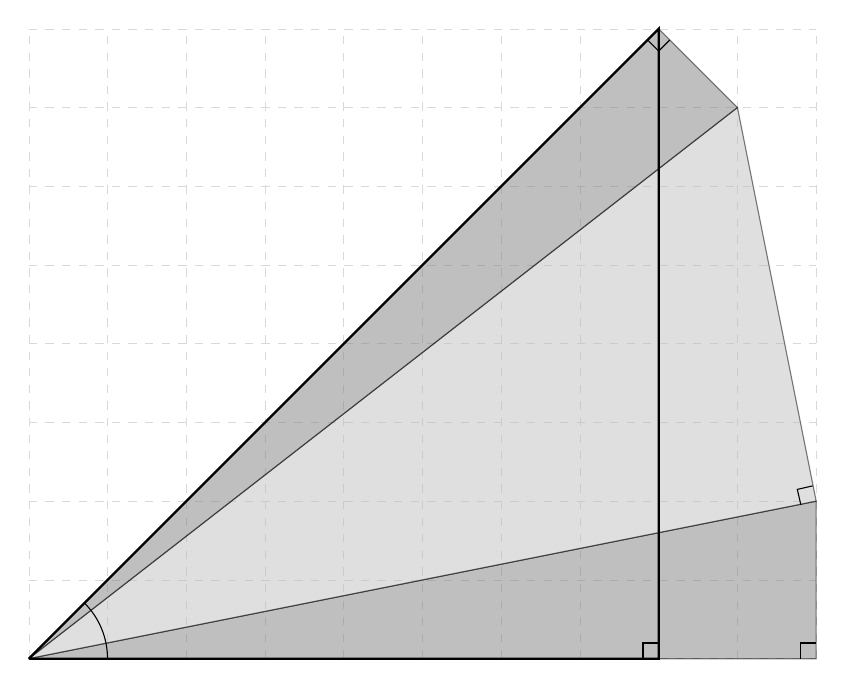
\begin{tikzpicture}
		\draw[help lines, color=gray!30, dashed] (0,0) grid (10,8);
		\draw[-,fill=gray, opacity=0.5] (0,0) -- (10,0) -- (10,2) -- (0,0);
		\draw[-,fill=gray!50!white, opacity=0.5] (0,0) -- (10,2) -- (9,7) -- (0,0);
		\draw[-,fill=gray, opacity=0.5] (0,0) -- (9,7) -- (8,8) -- (0,0);
		\draw[-,thick] (0,0) -- (8,0) -- (8,8) -- (0,0);
		\draw[rotate=-45] (0,1) arc (90:45:1);
		\draw[-] (9.8,0) -- (9.8,0.2) -- (10,0.2);
		\draw[-] (7.8,0) -- (7.8,0.2) -- (8,0.2);
		\coordinate(A) at (10,2);
		\coordinate(B) at (8,8);
		\draw[-,rotate around={13:(A)}] (10,2.2) -- (9.8,2.2) -- (9.8,2);
		\draw[-,rotate around={315:(B)}] (8.2,8) -- (8.2,7.8) -- (8,7.8);
	\end{tikzpicture}
\end{document}
